\chapter{Définition et mise en oeuvre d'un système de SLAM en temps-réel}

\section{De l'expression du besoin à une spécification complète}

  \subsection{Vision et cas d'utilisation}

Les réalisations effectuées ont été guidées par une phase d'analyse du besoin, menée de concert avec les membres de l'équipe projet. 
En qualité de tuteur de stage, M. David Daumand a guidé ce projet afin que le système final implique des perspectives commerciales concrètes. 
Dans cette optique, il a apporté son expertise sur ce que seraient les besoins de clients potentiels, en orientant la démarche vers une application militaire. 
Il a ainsi défini la dénomination du système \gls{SRT2M}, permettant à elle seule d'exprimer la fonction, le contexte et le secteur visé par le produit.  

La preuve de concept réalisée durant ce stage est un sous-système de \gls{SRT2M}. 
Afin d'en exposer clairement le périmètre, la figure \ref{fig:use-case} défini sa nomenclature et en donne les principaux cas d'utilisation. 

\begin{figure}[h]
  \centering
    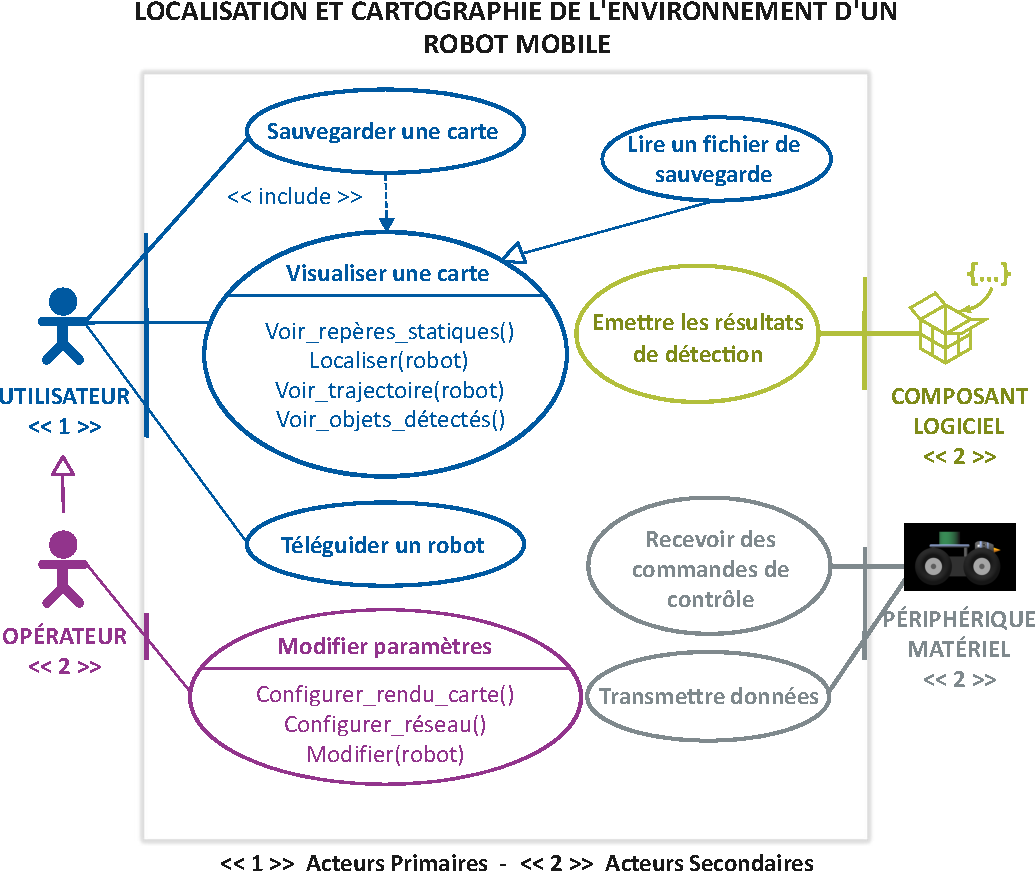
\includegraphics[width=.8\linewidth]{figures/use-case}  
  \captionof{figure}{Diagramme de cas d'utilisation du système de cartographie et de localisation d'un robot mobile}
  \label{fig:use-case}
\end{figure}

Ainsi, ce \emph{sous-système} doit permettre d'effectuer une cartographie de l'environnement d'un robot mobile, tout en donnant sa localisation. 
L'acteur primaire du système pourra visualiser une carte, soit à partir de données préalablement sauvegardées au sein de ce même système, soit grâce à des données acquises en temps réel par des périphériques dédiés. 
Cette visualisation implique la représentation d'obstacles statiques dans l'espace exploré, mais aussi la position et la trajectoire du robot en tout temps.
Le téléguidage du robot par l'utilisateur doit également être assuré. 
Un opérateur --typiquement un contributeur du système-- pourra jouer sur les paramètres de présentation des résultats, de la mise en réseau des périphériques ou de la définition de ces périphériques. 

Les périphériques matériel sont à ce stade réunis en un seul acteur ``Périphérique matériel''.
Il inclut le LIDAR et le robot qui permettent respectivement d'acquérir les mesures de distances aux obstacles et de déplacer la plateforme.
On souligne aussi la présence d'un ``Composant logiciel'' qui interagit avec le système.
Ce composant est vu comme une boîte noire qui fournit en sortie les résultats de détection et de classification d'objets d'intérêt rencontrés par le système.
Dans les faits, ces résultats correspondent à la position, la taille et la \gls{classe} de chaque objet, ce qui nous permettra de les représenter sur la carte générée (cf. fonction \path{Voir_objets_detectes()}).

\subsection{Formalisation d'exigences}

\begin{figure}[h]
  \centering
    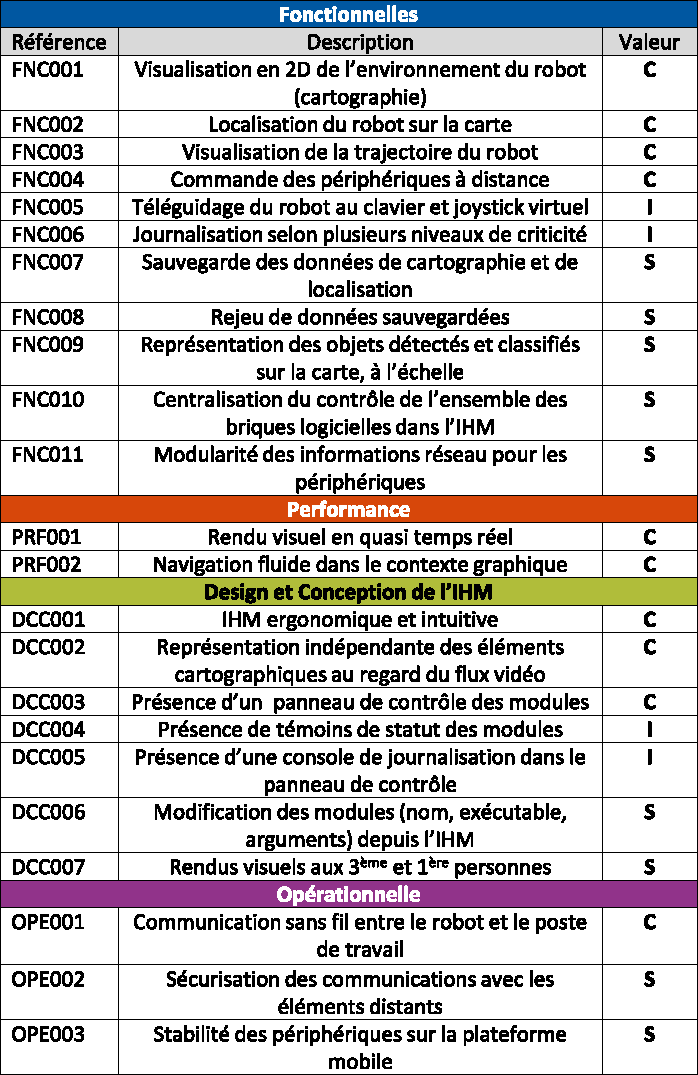
\includegraphics[width=.65\linewidth]{figures/exigences}  
  \captionof{figure}{Exigences de Spécification Technique du Besoin Logiciel}
  \label{fig:exigences}
\end{figure}

Les réalisations s'articulent autours d'exigences formalisées au sein d'un document de spécification du besoin logiciel (\gls{STBL}) dont le but et la portée seront décrits dans la section \nameref{sec:orga}.
La figure \ref{fig:exigences} reprend les déclarations de haut-niveau qui permettent de cerner les principaux axes de l'analyse fonctionnelle. 
Les exigences exposées s'appliquent à un ou plusieurs composants du système\footnote{Par opposition aux exigences unitaires --allouées à un et un seul composant-- abordées au chapitre \nameref{chap:bilan}}. 
  
Chaque exigence est une entrée du tableau, que l'on associe à l'une des catégories suivantes : 

\begin{itemize}
 \item \textbf{fonctionnelle} réuni les besoins métiers qui justifient la réalisation du logiciel
 \item \textbf{performance} regroupe les contraintes spécifiques liées au temps d'exécution ou à l'utilisation des ressources 
 \item \textbf{design et conception} donne les impératifs en termes de rendu visuel
 \item \textbf{opérationnelle} traite des interactions survenant pendant l'exploitation du système
\end{itemize}

On attribue une référence unique permettant le suivi unitaire des exigences lors des différentes phases du projet, une description textuelle non ambigüe ainsi que le niveau de criticité de l'exigence :
``C'' signifie critique, ``I'' important et  ``S'' souhaitable. 

\`{A} ce niveau, les exigences ne suggèrent pas d'implémentation ou de choix techniques. 
Par contre, elles guident l'ensemble de la réalisation, depuis la conception jusqu'aux tests, en passant par l'estimation de la satisfaction du client. 
Chacune d'entre-elles s'accompagne donc d'un paragraphe servant à la détailler, à en donner les pré-requis et les cas de validation.
Par exemple, on précisera que la FNC001 nécessite la possession d'un matériel d'acquisition de mesures spatiales ou, à défaut, de données de test simulant cette acquisition. 

Dans ce qui va suivre, nous nous concentrerons sur les exigences qui apportent la valeur intrinsèque de l'ouvrage, en mettant l'accent sur les niveaux de criticité élevés : à savoir celles qui 
permettent d'établir et de représenter une cartographie de l'espace et d'y localiser le robot en tout temps. 
La définition de ces exigences a permis d'entamer une phase de définition des architectures physique et logicielle sereinement, sans perdre de vue l'ensemnle des fonctionnalités à assurer et leur priorité respective. 

  \subsection{Matériel et Interfaces}
  \label{subsec:archi-physique}
  
Les fonctionnalités principales de l'application dépendent de l'acquisition de mesures spatiales. 
Ainsi, nous devions nous doter d'une dispositif capable de prendre ces mesures et de les relayer en quasi temps-réel jusqu'à un module de traitement, encore à définir. 

\begin{figure}[h]
  \centering
    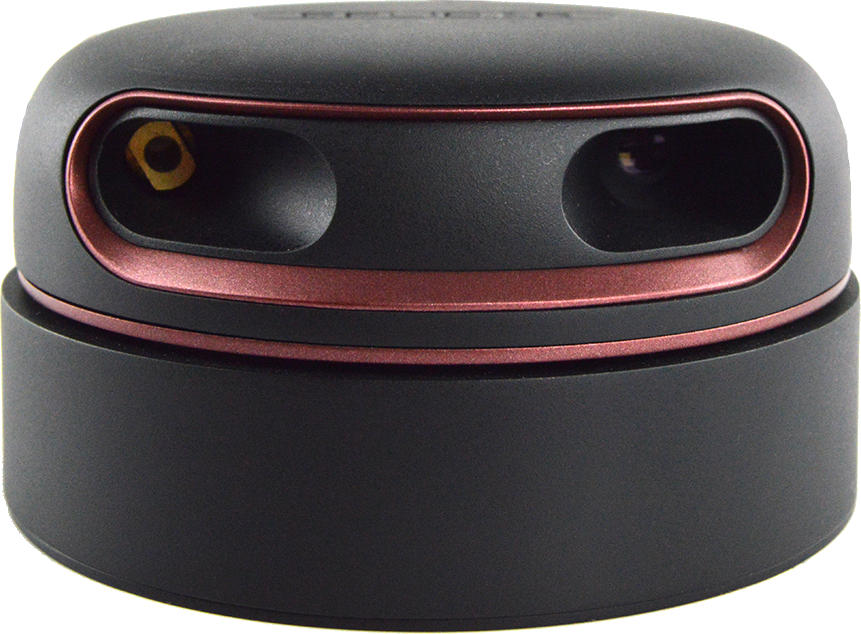
\includegraphics[width=.2\linewidth]{figures/rplidar_a2}  
  \captionof{figure}{RPLidar A2 utilisé durant le projet, développé par SLAMTEC}
  \label{fig:rplidar}
\end{figure}

Le choix du matériel retenu a fait l'objet d'une veille technologique visant à comparer les différents \gls{LIDAR} présents sur le marché. 
Ceux-ci ont pu être classés, outre selon leur prix, selon les critères suivants : 

\begin{itemize}
  \item la technologie employée (1D, 2D, 3D)
  \item la documentation disponible (notamment en ce qui concerne l'utilisation de la \gls{SDK})
  \item la précision angulaire
  \item la vitesse de calcul et de transfert des mesures
  \item la pérennité du produit et/ou de la marque en gage de qualité
  \item la disponibilité du produit en France, selon des délais serrés
\end{itemize}

Le résultat de ce comparatif a débouché sur l'acquisition du RPLidar A2 visible sur la figure \ref{fig:rplidar}.
Celui-ci est équipé d'un seul faisceau laser qui a la particularité de tourner sur 360\degre. 
Cet équipement est donc adapté à la mesures des distances dans un espace plan, tout en impliquant une dépense acceptable. 
\begin{figure}[h]
  \centering
    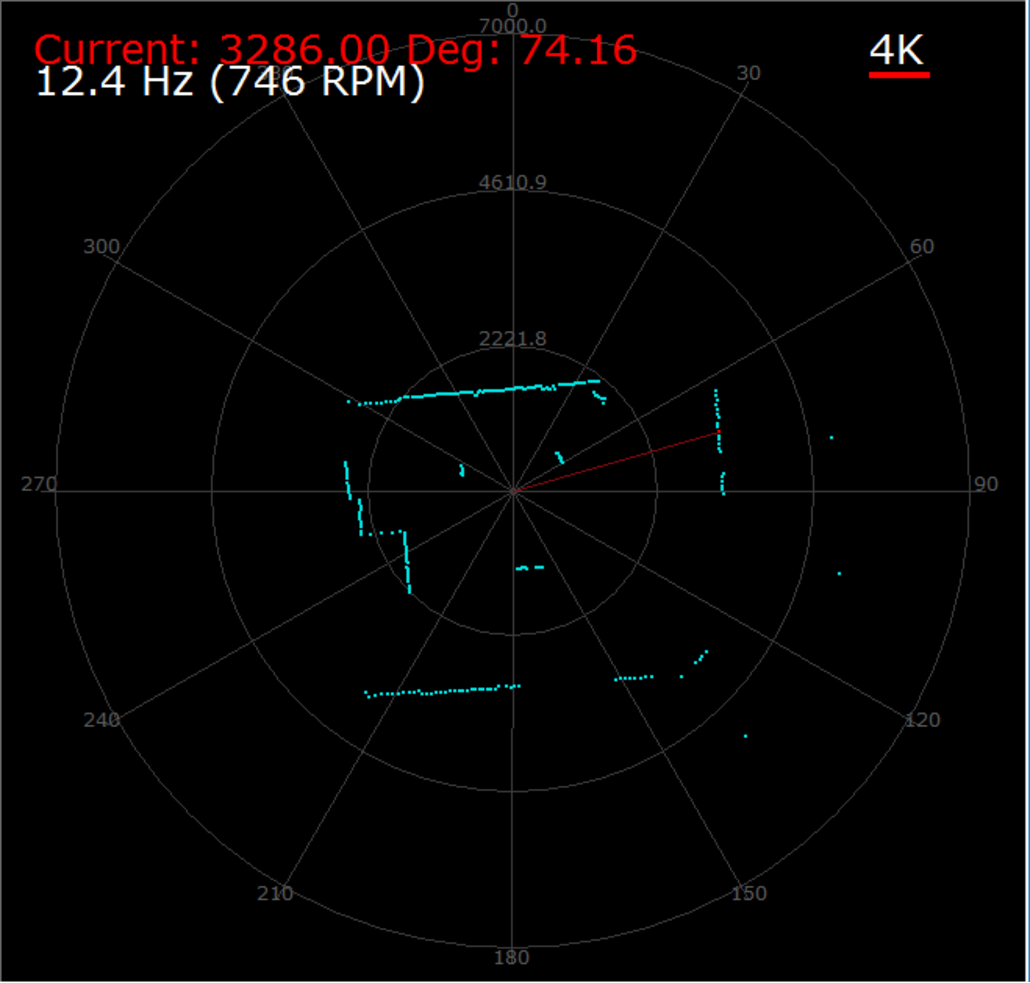
\includegraphics[width=.5\linewidth]{figures/lidar-points}  
  \captionof{figure}{Résultats de l'application constructeur du RPLidar A2}
  \label{fig:lidar-points-cloud}
\end{figure}
La possibilité d'équiper le robot de servo-moteurs et d'un LIDAR à faisceau unique fixe moins onéreux a également été explorée, mais n'a pas été retenue au regard de la compléxité de mise en \oe{}uvre d'un tel dispositif, 
du coût cumulé du LIDAR et des servo-moteurs et enfin, des fortes imprécisions potentiellement engendrées lors du mouvement du robot. 
La figure \ref{fig:lidar-points-cloud} montre le nuage de points restitué par un logiciel intégré au kit de développement du LIDAR, utilisable sous Windows.  

Par ailleurs, le robot mis à disposition du projet est un Wifibot Lab v3, muni d'une carte mère Windows Embedded. 
Enfin, un nano-ordinateur Raspberry Pi 3 modèle B est utilisé à des fins de communication entre les briques embarquées et une station de travail qui réuni les modules de calcul et l'\gls{IHM}.

Nous obtenons ainsi l'archtecture physique schématisée sur la figure \ref{fig:archiphy}, au travers de laquelle sont définis quatre modules principaux, notés $M_{i}$.

\begin{figure}[h]
  \centering
    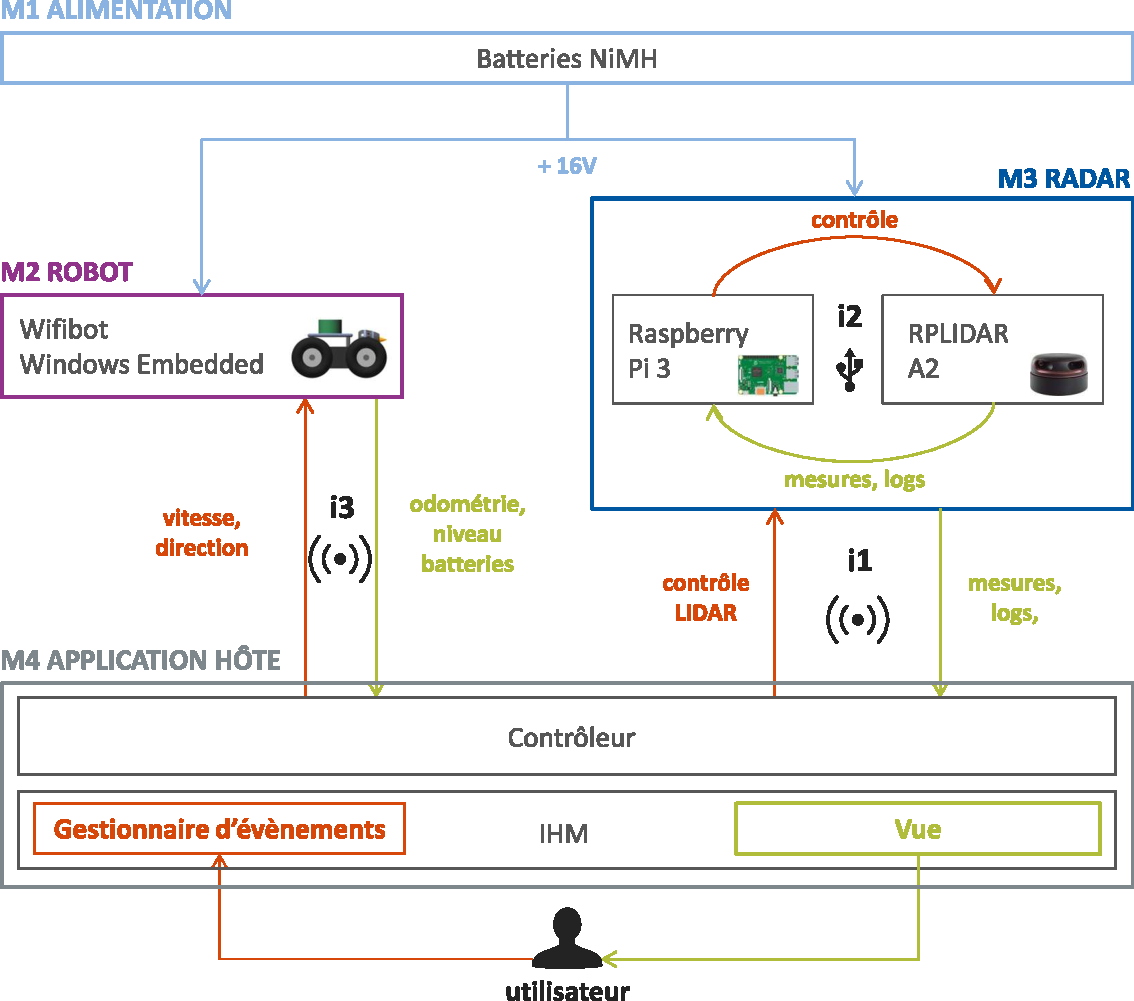
\includegraphics[width=.9\linewidth]{figures/archi-phy}  
  \captionof{figure}{Architecture physique du projet}
  \label{fig:archiphy}
\end{figure}

$M_{1}$ est dédié à l'alimentation électrique du robot, du LIDAR et du Raspberry Pi.
$M_{2}$ correspond au Wifibot, $M_{3}$ regroupe le LIDAR et le Raspberry Pi et $M_{4}$ symbolise l'application hôte sur une station de travail Linux
\footnote{Ce dernier module présente un intérêt seulement en termes de transmission de données avec les périphériques matériels}.

Les interactions entre les briques matérielles sont représentées par des flèches d'entrées / sorties ou internes aux modules, représentées de la couleur orange quand il s'agit de requêtes et de la couleur verte pour 
les répo,ses afférentes. 
Par ailleurs, des interfaces de communications inter-modules notées $i_{i}$ apparaissent en noir et définissent les canaux au travers desquels requêtes et réponses sont transmises. 

L'application hôte est responsable de l'émission de commandes de contrôle du LIDAR au travers d'une interface WiFi\footnote{Le Raspberry Pi 3 est nativement doté d'une carte et d'un émetteur WiFi} $i_{1}$. 
Ces commandes transitent par le Raspberry Pi 3 qui les formattera et les transmettra au LIDAR via la liaison USB $i_{2}$. 
Ce cheminement de données peut être parcouru dans le sens inverse pour remonter les données acquises par le LIDAR à savoir, 
des mesures de distances spatiales, communiquées tous les 360\degre, pouvant être perçues comme des nuages de points. 

Parallèlement, $M_{4}$ communique directement des ordres de vitesse et de direction au Wifibot à travers de l'interface WiFi $i_{3}$. 
Ces commandes de direction sont quasi-instantanément suivies de réponses contenant les relevés odométriques des encodeurs du Wifibot, son niveau de batterie et le relevé de capteurs infrarouges présents 
à l'avant du robot. Les réponses empruntent là encore le chemin inverse par le biais de la même interface. 

\section{Théorie et choix techniques}

  \subsection{Cartographie et Localisation Simultannées}
  
Le SLAM, pour Simultaneous Localization And Mapping, est un ensemble de méthodes permettant à un robot mobile d'établir une cartographie de son environnement et de se repérer de manière fiable dans cette même carte. 
 
De manière générale, on peut dégager un schéma autours duquel s'articulent ces techniques, dont la figure \ref{fig:slam-proc} donne les grandes lignes.

\begin{figure}[h]
  \centering
    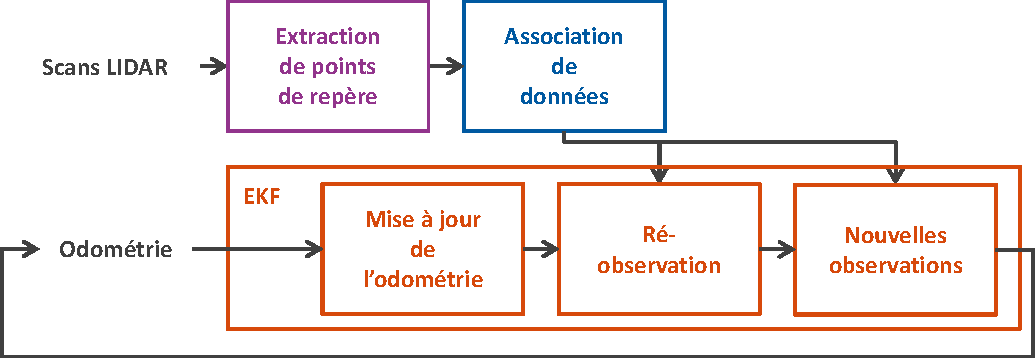
\includegraphics[width=.8\linewidth]{figures/slam-proc-h}  
  \captionof{figure}{Architecture physique du projet}
  \label{fig:slam-proc}
\end{figure}

La première étape d'un processus de SLAM consiste à récupérer les données numériques issues d'un laser. 
Généralement, on peut décrire de telles données en termes de précision, de champs de capture, de longueur du faisceau ou encore de résolution verticale. 
Le RPLidar A2 dispose d'un champ de 360\degre sur l'axe horizontal (scan plan), d'une fréquence de rotation typique autour de 600 rpm, d'une portée comprise entre 0.15 et 6m et pour finir, d'une résolution angulaire comprise entre 
0.45\degre et 1.35\degre.

Les données odométriques (ou odométrie) permettent la prédiction de la position du robot dans le plan. 
Ce calcul se base généralement sur les relevés de capteurs internes au robot (différentiel de vitesse entre les deux roues motrices, donné par des encodeurs internes). 
La difficulté réside lorsqu'il s'agit de corréler dans le temps et avec précision ces données, avec les mesures en sortie du laser.
Pour pallier ce problème, l'odométrie peut être extrapolée de l'instant précédant dans une démarche prédictive. 

Une fois les données externes collectées, il convient de les traiter pour en extraire des \gls{landmarks} spatiaux. 
Cette étape, représentée en violet sur la figure \ref{fig:slam-proc}, consiste à caractériser les points de repère pertinents. 
Ils sont ensuite gardés en mémoire pour établir la cartographie de l'espace et également en vue d'être discriminés ou assimilés ultérieurement.
Plusieurs algorithmes, tels que Spike ou RANSAC, proposent ces fonctionnalités avec des approches diverses qu'il convient d'adapter à une application donnée\cite{Bib_dummies}.

L'étape suivante, représentée en bleu sur la figure \ref{fig:slam-proc}, vise à associer les données collectées, à savoir reconnaitre les points de repère qui arrivent dans le champs d'observation du robot à plusieurs reprises. 
Le problème de l'association de données vise à prendre en compte du mieux possible les risques de confusion ou de non reconnaissance de points de repères au travers d'une politique de validation qui encadre la fusion de données. 
\`{A} cet effet, on peut appliquer l'algorithme \gls{KNN} implémentant des mesures de distances diverses comme la distance Euclidienne ou la distance de Maahalanobis.

Enfin, le filtre de Kalman étendu est utilisé pour estimer un vecteur d'état du robot (à savoir sa position et son orientation).
Dès lors que les briques d'extraction de points de repère et d'association de données sont mises en place, un processus de SLAM peut être considéré en trois étapes, présentées en orange sur la figure \ref{fig:slam-proc}. 
Le premier point consiste simplement à ajouter les relevés odométriques du robot à l'ancien vecteur d'état. 
Le deuxième point apporte une correction au vecteur d'état et à l'état du système de façon globale.
En effet, au vu de l'état courant, on peut estimer la position des points de repère précédemment selectionnés.
Si un décalage spatial a lieu, on l'appellera innovation, c'est-à-dire la différence entre la position estimée du robot à l'étape 1 et sa position basée sur la perception de son environnement.
De plus, cette étape nous permettra d'affiner la confiance accordée dans notre connaissance de l'environnement. 
Une innovation faible va entraîner une confiance accrue quant aux positions des points de repère connus et visible, tandis qu'une innovation forte aura l'effet inverse.
Le troisième point permet d'ajouter à notre système les points de repère détectés ayant été discriminés par la politique d'association mise en place. 

La définition et l'implémentation d'un algorithme de SLAM est un processus fastidieux qui repose sur des fondements théoriques complexes. 
La diversité de ces algorithmes\cite{Bib_openslam} dénote l'ampleur de la tâche qui consiste à les recenser, à en comprendre tous les rouages pour proposer des améliorations et finalement passer à l'implémentation. 
Ainsi il n'était pas envisageable de développer un algorithme de SLAM dédié au projet. 
Par contre, l'utilisation de tels algorithmes paraissait incontournable au regard des exigences du projet. 
Un état de l'art sur le sujet a donc été mené, permettant de choisir l'algorithme à intégrer, présenté à la section \ref{subsection:hector}. 

  \subsection{Le méta-système d'exploitation ROS}

\begin{figure}[h]
  \centering
    
\includegraphics[width=.2\linewidth]{figures/ros_logo}  
  \captionof{figure}{Logo du méta-système d'exploitation ROS (issu du kit de presse ROS\cite{Bib_ROS})}
  \label{fig:ros}
\end{figure} 
  
Robot Operating System, ou \gls{ROS}, est un middleware pour systèmes Unix destiné à la réalisation de projets robotiques écrits en C++ ou en Python.
Il offre des fonctionnalités liées à la robotique grâce à des librairies dédiées mais aussi des moyens de communication et des outils facilitant le développement et le déploiement de tels systèmes. 
Il a ainsi été rapidement étudié puis adopté pour ce projet sous sa version Kinetic. 
Notre utilisation de \gls{ROS} couvre les briques logicielles embarquées sur le Raspberry Pi et des briques présentes localement sur le poste de travail de l'utilisateur final. 
Son fonctionnement passe par la création d'un réseau de n\oe{}uds\cite{Bib_ROS_nodes}, c'est-à-dire des exécutables dans l'écosystème \gls{ROS}, organisés autour d'un n\oe{}ud central appelé \gls{ROS} Master\cite{Bib_ROS_master}.
Cette entité enregistre les noeuds, leur fourni un nom et instancie un annuaire qui leur permet d'échanger des données. 
Il s'appuie en partie sur le protocle \gls{XMLRPC}.

Les noeuds disposent de plusieurs moyens de communication, disponibles à travers une librairie cliente fournie par \gls{ROS} : les \gls{topics}\cite{Bib_ROS_topics} auxquels il est possible de s'abonner, 
les \gls{services}\cite{Bib_ROS_services} qui fonctionnent sur le modèle requête / réponse, et des valeurs stockées par un \gls{serveur de parametres} géré par le \gls{ROS} master et qui peuvent être récupérés par les noeuds durant leur exécution.
On notera que, dans le cas des topics, le format des données transmises correspond généralement à des types de messages définis par \gls{ROS} dans ses packages 
internes\footnote{Lors d'une installation standard, ces paquets se situent sous \path{/opt/ros/<ROS-version>/share/} pour les messages et \path{/opt/ros/<ROS-version>/include/} pour les fichiers d'en-tête}. 
Par exemple, le type de données \path{sensor_msgs/LaserScan} dispose d'un fichier de définition du même nom, portant l'extension \path{.msg} et d'un fichier d'en-tête qui permet la publication et l'abonnement aux topics 
de ce type.
\`{A} titre d'exemple, le fichier \path{sensor_msgs/LaserScan.msg} est présenté en \nameref{annexe:laserscan}.

Le framework s'accompagne de nombreux utilitaires en ligne de commande qui permettent à l'utilisateur de configurer le réseau, de le sonder et de créer des noeuds à la volée pour diverses utilisations.

\gls{ROS} dispose également d'un outil de gestion du système de fichiers et de cha\^{i}ne de compilation nommé \gls{Catkin}.
Ce dernier permet la mise en place d'un format d'arborescence facilitant la production et la gestion de packages.
Ces packages sont définis comme des agglomérats logiques de n\oe{}uds et possèdent une structure spécifique au sein de l'environnement de travail \gls{Catkin}, tel que représenté ci-dessous. 
\\
\renewcommand*\DTstylecomment{\rmfamily\color{red}}
\dirtree{%
.1 catkin\_workspace/\DTcomment{racine de l'environnement catkin}. 
.2 src/\DTcomment{emplacement des codes sources}. 
.3 CMakeLists$.$txt\DTcomment{invoqué par CMake lors de la configuration de l'environnement}. 
.3 package\_1/. 
.4 CMakeLists$.$txt\DTcomment{invoqué par CMake lors de la compilation de package\_1}. 
.4 package$.$xml\DTcomment{manifeste du package\_1}. 
.4 default$.$launch\DTcomment{fichier de lancement des n\oe{}uds du paquet}. 
.4 src/\DTcomment{contient les sources du paquet, implémentant un ou plusieurs n\oe{}uds}. 
.3 package\_2/. 
.4 CMakeLists$.$txt. 
.4 package$.$xml. 
.4 src/. }

Le fichier package.xml\cite{Bib_ROS_package} est le manifeste des paquets. Placé à la racine de chacun d'entre-eux, il en donne la définition (nom, version, auteur, license) ainsi que les dépendances. 
Les fichiers CMakeLists.txt\cite{Bib_ROS_manifeste} sont les entrées du système de build CMake, invoqués dans la chaîne de compilation de catkin. 
C'est ici que l'on définit les noms et fichiers sources associés à chaque n\oe{}ud du paquet, les sources étant généralement stockées sous le répertoire \path{catkin_workspace/src/<package_name>/src/}. 
L'\nameref{annexe:catkindocs} permet d'illustrer le formalisme de ces deux documents. 

Les deux éléments précédents sont indispensables à la création de paquets dans l'environnement catkin. 
Parallèlement, on relève la présence d'un fichier portant l'extension \path{.launch}, appelé launchfile.  
Ce fichier optionnel permet d'exécuter, via un utilitaire en ligne de commandes, plusieurs n\oe{}uds en une seule fois. 
Pour parser et exécuter le launchfile présent dans notre exemple on saisira simplement :
\\
\begin{lstlisting}[style=customcpp]
> roslaunch package_1 default.launch
\end{lstlisting}


Les briques logicielles implémentées avec \gls{ROS} présentent intrinsèquement un fort potentiel de modularité et de maintenabilité. 
En effet, chaque package et chaque n\oe{}ud observent des cycles de vie indépendants et n'interagissent les uns avec les autres qu'en cas d'échange d'informations utiles. 
Cet aspect modulaire, sur lequel nous reviendrons, a fortement participé à l'adoption de \gls{ROS} et de ses outils. 
De plus, \gls{ROS} est un outil entretenu par une large communauté de chercheurs et développeurs qui alimentent fréquemment l'écosystème par de nouveaux paquets, généralement mis à l'épreuve lors de compétitions robotiques internationales. 
Ainsi, la problématique de \gls{SLAM} est largement couverte par \gls{ROS}, tant et si bien que les librairies et outils publics dédiés au \gls{SLAM} se retrouvent presque exclusivement sous la forme de paquets \gls{ROS}.

  \subsection{Hector SLAM}
  \label{subsection:hector}
  
Dans le cadre de ce projet un état de l'art a été entrepris, visant à recenser les principaux algorithmes de \gls{SLAM} intégrables à notre système logiciel.
Les algorithmes majeurs du domaine ont donc été étudiés et qualifiés notamment au travers des applications qu'ils visent, de leur principe de fonctionnement, des possibles implémentations qu'elles connaissent et de leurs limites. 
Suite à cette étude, le projet \gls{Hector SLAM} a été retenu. 
Notons qu'il profite d'une notoriété acquise depuis plusieurs années, lui permettant d'être aujourd'hui encore largement actif et reconnu\cite{Bib_Hector_2016}\cite{Bib_Team_Hector}. 

\gls{Hector SLAM} est un métapackage\footnote{Un métapackage est simplement pourvu d'un manifeste qui permet de référencer des paquets regroupés logiquement mais faiblement couplés d'un point de vue fonctionnel}
\gls{ROS}\cite{Bib_Hector_git} qui inclut nativement trois packages principaux : \path{hector_mapping}, \path{hector_geotiff} et \path{hector_trajectory_server}. 
Nous ne reviendrons pas sur \path{hector_geotiff} responsable de l'enregistrement des données au format \gls{GeoTIFF} qui a été écarté du système final. 
\path{hector_mapping} est le moteur de \gls{SLAM} intégré par Hector. Il a la particularité de ne pas requérir de données odométriques pour fonctionner. 
Cela sous-entend que l'on peut disposer de résultats de SLAM en tenant simplement le LIDAR dans ses mains.
Ce point a été déterminant dans la sélection d'\gls{Hector SLAM} puisque d'une part l'acquisition du robot s'est faite tardivement, 
et d'autre part, ce dernier a été fourni sans documentation permettant de s'assurer de la précision des encodeurs. 
Nous avons donc préféré un système de \gls{SLAM} qui favorise les données issues du \gls{LIDAR} fraîchement acquis. 
Par ailleurs, \gls{Hector SLAM} s'adapte à une utilisation sur des drônes par le biais de données \gls{IMU}. 
Dans l'optique d'assurer une continuité au projet en l'orientant vers le secteur de la défense, la possibilité d'adapter le système à des dispositifs aériens semblait particulièrement intéressante. 
Enfin, le n\oe{}ud \path{/hector_trajectory_server} est utilisé pour traiter la succession de positions de la plateforme mobile depuis le début de l'acquisition. 

\begin{figure}[h]
  \centering
    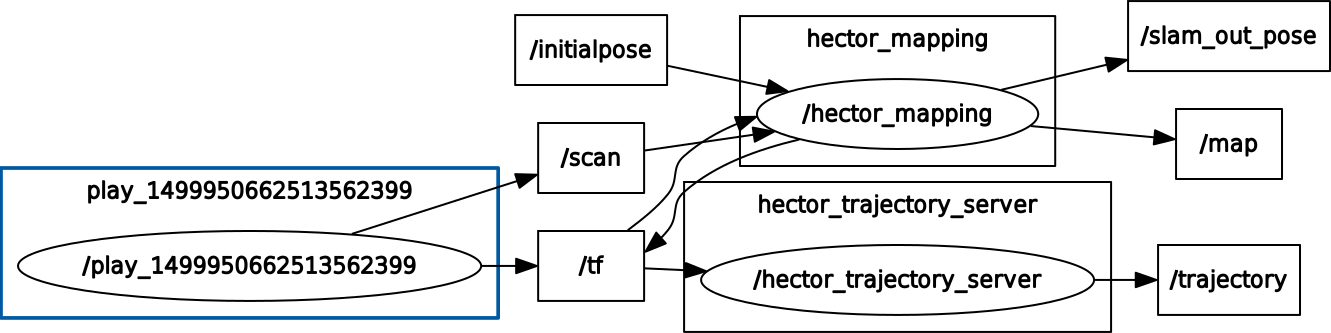
\includegraphics[width=1.\linewidth]{figures/hector_active_nodes}  
  \captionof{figure}{N\oe{}uds et topics d'intérêt et actifs lors de l'exécution d'Hector SLAM}
  \label{fig:hector}
\end{figure}

La figure \ref{fig:hector} expose les n\oe{}uds et topics actifs lors d'un l'utilisation d'\gls{Hector SLAM} à partir d'un jeu de données pré-enregistrées dans un fichier \gls{bagfile}.
Les n\oe{}uds actifs sont présentés au sein d'ellipses, les topics au sein de rectangles sous la forme \path{/<topic-name>} et les noms des packages auxquels les n\oe{}uds appartiennent figurent au dessus de chacun d'entre-eux. 
Enfin, les flèches signalisent quels sont les n\oe{}uds responsables de la publication des topics, et quels sont les n\oe{}uds qui s'y sont inscrits. 
Le package généré par la lecture du \gls{bagfile} est représenté en bleu. 

On s'intéresse particulièrement aux topics en sortie d'\gls{Hector SLAM}. 
\path{/slam_out_pose} donne la localisation du robot en terme de position et d'orientation, \path{/trajectory} définit la trajectoire parcourue par le robot et \path{/map} donne la représentation de son environnement. 
Ce dernier topic correspond à une grille d'occupation, à savoir une discrétisation de l'espace sous forme de grille où chaque case porte la probabilité qu'elle soit un obstacle.
Dans la pratique la carte est de dimensions $2048 \times{2048}$ avec une résolution de $0.05m$. Les résultats issus de l'approche probabiliste s'expriment selon trois valeurs : $0$ pour une case vide, $1$ pour une case occupée et $-1$ pour une case inconnue. 
Chaque nouvelle acquisition attestant l'occupation d'une case augmente sa probabilté, et inversement lorsqu'une acquisition démontre que la case est libre.
Lorsque la probabilité portée par une case dépasse un seuil interne à \gls{Hector SLAM}, la case sera considérée comme occupée et passera à la valeur $1$\footnote{Ce seuil est fixé à $0.5$}

L'intégration d'\gls{Hector SLAM} au projet s'est déroulée en plusieurs temps.
Nous avons d'abord pu prendre l'outil en main avant l'achat du \gls{LIDAR} grâce à l'utilisation de données de test contenues par des \gls{bagfile}. 
Durant cette étape, les résultats pouvaient être visualisés grâce à RViz, un outil graphique inclu dans \gls{ROS}\footnote{Pour la distribution Kinetic de ROS, RViz est présent dans les paquets d'installation dits ``Desktop''\cite{Bib_ROS_install}.}.
La figure \ref{fig:rviz} illustre le résultat obtenu pour un jeu de test issu de la RobotCup German Open 2011. 
Dans un deuxième temps, il a fallu adapter \gls{Hector SLAM} pour recevoir en entrée les données du \gls{LIDAR}, ce qui revient principalement créer des fichiers de lancement (\emph{launchfile})
adaptés au périphériques d'acquisition. Dans notre cas nous avons créé deux fichiers distincts : l'un pour le mode d'exécution standard et l'autre pour un mode ``degub''.
Nous avons également mis en place des éléments qui définissent les tranformations spatiales entre les différents périphériques matériels et qui seront évoqués dans la partie \ref{subsection:ROSnodes}. 

\begin{figure}[h]
  \centering
    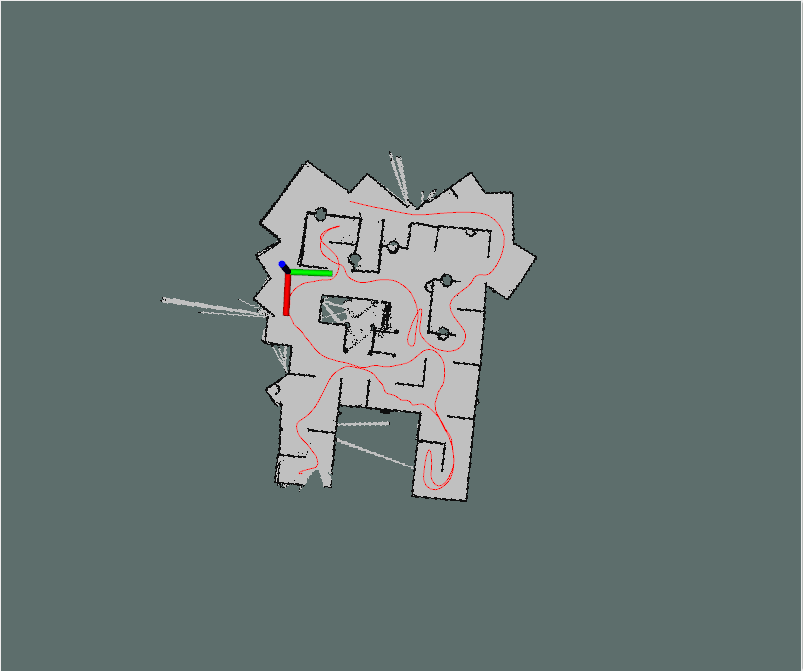
\includegraphics[width=.4\linewidth]{figures/rviz}  
  \captionof{figure}{Visualisation avec RViz d'un jeu de données pré-enregistrées}
  \label{fig:rviz}
\end{figure}

Sur la figure \ref{fig:rviz}, les zones non explorées figurent en gris foncé, les zones explorées mais vides en gris clair et les zones occupées en noir. 
Le robot est resprésenté par trois composantes orthogonales de couleur bleue, verte et rouge et la trajectoire parcourue est une courbe rouge. 

\section{Réalisations et architecture logicielles}

  \subsection{Le réseau ROS complet}
  \label{subsection:ROSnodes}
  
\gls{Hector SLAM} a été intégré à un réseau plus large prennant en compte les spécificités de notre application. 
Il était entendu que l'\gls{IHM} ne serait pas inclue dans ce réseau et serait développée avec Qt Creator (voir partie \ref{subsection:Qt}).  

La définition du réseau doit alors s'inscrire comme une solution aux problématiques suivantes : 

\begin{itemize}
  \item le contrôle du \gls{LIDAR} ainsi que la lecture et l'émission des nuages de points calculés
  \item l'intégration d'\gls{Hector SLAM} 
  \item la communication des résultats de cartographie et de localisation vers l'\gls{IHM}
\end{itemize}

\begin{figure}[h]
  \makebox[\textwidth][c]{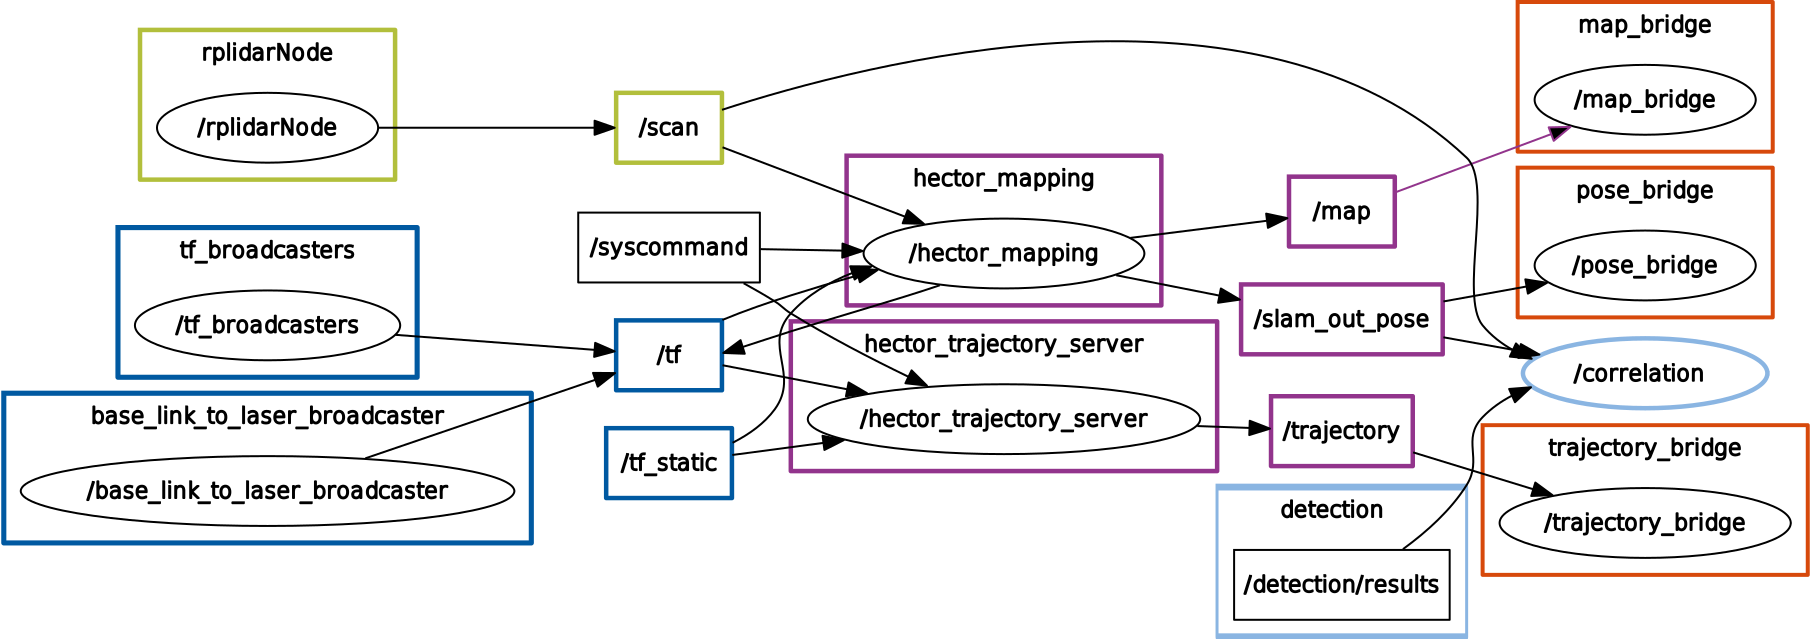
\includegraphics[width=1.1\textwidth]{figures/all_nodes}}%
  \captionof{figure}{Réseau ROS intégré au système}
  \label{fig:rosnet}
\end{figure}

Le premier point, représenté en vert sur la figure \ref{fig:rosnet}, est assuré par un n\oe{}ud embarqué sur le Raspberry Pi régissant la communication avec le \gls{LIDAR}.   
Il s'interface avec plusieurs fichiers d'en-tête qui constituent la \gls{SDK} du \gls{LIDAR}.
Cet élément du réseau \gls{ROS} est fourni par le constructeur du \gls{LIDAR} dans son kit de développement.
Sa mise en \oe{}uvre a demandé de comprendre les principales méthodes de la \gls{SDK} et la portée fonctionnelle de chaque fichier d'en-tête. 
Par ailleurs, outre l'installation de \gls{ROS} sur Raspberry, la mise en place du matériel a nécessité l'installation d'un driver permettant la conversion des données 
depuis un l'UART vers l'USB, ainsi que la définition de règles d'utilisation du port série sur lequel est raccordé le \gls{LIDAR}.
En sortie, ce n\oe{}ud publie le topic \path{/scan}, correspondant au format de messages \path{sensor_msgs/LaserScan} précédemment évoqué. 

\begin{figure}[h]
  \centering
    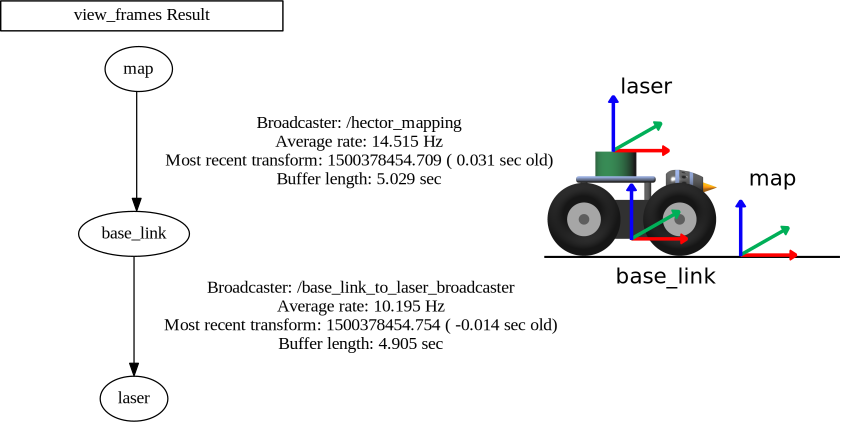
\includegraphics[width=1.\linewidth]{figures/frames_and_schema}  
  \captionof{figure}{Systèmes de coordonnées et transformations au sein du système}
  \label{fig:frames}
\end{figure}

L'intégration d'Hector SLAM demande la définition de plusieurs systèmes de coordonnées correspondant au divers composants du système.
Les transformations spatiales entre ces systèmes étant également requises par \gls{Hector SLAM}, elles sont publiées au travers d'un package appelé \gls{tf}\cite{Bib_ROS_tf}\cite{Bib_tf}. 
Les n\oe{}uds et topics impliqués dans ce processus sont représentés en bleu foncé sur la figure \ref{fig:rosnet}. 
\gls{tf} distingue deux types de transformations : les transformations statiques et les transformations dynamiques. 
Dans le premier cas, il suffit de définir l'identifiant d'un repère de référence (\emph{frame\_id}) et d'un repère fils (\emph{child\_frame\_id}) ainsi que la transformation que subit ce dernier, en s'assurant qu'il ne sera jamais amené à changer.
Dans le second cas, il faut généralement passer par la création d'un noeud publiant la valeur de ce décallage régulièrement durant l'exécution. 
Pour mieux saisir les enjeux soulevés par l'intégration d'\gls{Hector SLAM}, la figure \ref{fig:frames} donne les systèmes de coordonnées définis, 
ainsi que les n\oe{}uds implémentés (les \emph{broadcasters}) responsables de la publication des transformations. 

Le système \emph{map} est un repère fixe, ancré au sol, qui sert de référence au positionnement du robot sur le long terme\cite{Bib_frames}.
\emph{base\_link} est un repère mobile par rapport à \emph{map} attaché sous la plateforme mobile en son centre. Une première transformation entre \emph{map} et \emph{base\_link} est requise par \gls{Hector SLAM}. 
Elle est calculée par le n\oe{}ud \path{/tf_broadcasters} (voir figure \ref{fig:rosnet}) à partir des relevés odométriques fournis par le robot.
Une fois intégrée par \gls{Hector SLAM}, cette transformation est corrigée puis ré-émise par \path{/hector_mapping} : c'est le topic \path{/tf} de la figure \ref{fig:rosnet}. 
Enfin, le n\oe{}ud \path{/base_link_to_laser_broadcaster} publie régulièrement la transformation entre \emph{base\_link} et \emph{laser}, c'est-à-dire le différentiel de position entre la base du robot et le \gls{LIDAR}. 
Celui-ci n'étant jamais amené à changer nous sommes dans le cas d'une transformation statique définie de la manère suivante dans le launchfile d'Hector SLAM en mode d'exécution 
standard\footnote{En mode ``debug'' cette transformation est non avenue puisqu'elle est déja comprise dans les données à rejouer, à savoir le bagfile} : 

\begin{lstlisting}[style=custombash]
<!-- Laser is set 25cm above robot base. Node arguments must be : 
dx dy dz yaw pitch roll frame_id child_frame_id publishing_frequency_in_ms 
-->

<node pkg="tf" type="static_transform_publisher" 
      name="base_link_to_laser_broadcaster" 
      args="0 0 0.25 0 0 0 base_link laser 100" />  
\end{lstlisting}

Nous obtenons ainsi un moteur de SLAM fonctionnel à partir duquel nous devons construire une \gls{IHM}. 
Pour ce faire, nous avons défini trois packages appelés \emph{bridges} représentés en orange sur la figure \ref{fig:rosnet}. 
Chacun d'entre-eux s'abonne à l'un des topics en sortie d'\gls{Hector SLAM}, 
Ensuite, les données utiles sont formatées par appel à une classe statique nommée \path{Serializer} et communiquées à l'\gls{IHM} par le biais d'un client \gls{TCP} implémenté avec l'API socket. 
La sérialisation répond à un schéma générique composé d'une en-tête (\emph{header}) et d'une charge utile (\emph{payload}). Il est représenté sur la figure \ref{fig:buffer}. 

\begin{figure}[h]
  \centering
    
\includegraphics[width=.5\linewidth]{figures/buffer}  
  \captionof{figure}{Définition du paquet générique de transmission de données à l'IHM}
  \label{fig:buffer}
\end{figure}

Les éléments contenus par le header sont \path{tID}, un identifiant donnant le type de la donnée transmise, \path{pSize}, la taille du payload et un \path{padding} à $0$ qui vise à ce que le \emph{header} atteigne 20 octets. 
La formation du \path{payload} dépend quant à elle des données à tansmettre. 
La principale difficulté réside en la transmission de la grille d'occupation contenue par le topic \path{/map}. 
Celle-ci contenant plus de $4 000 000$ de valeurs entières, nous nous sommes focalisé sur l'émission de mises à jour locales à chaque acquisition, plutôt que globales\footnote{Il en va de même pour la trajectoire où,
dans un même souci d'optimisation, nous effectuons un différentiel entre les valeurs précédemment acquises et la nouvelle acquisition}. 
Ainsi, le \path{payload} se construit de la manière suivante afin de désencombrer la bande passante et réduire la taille de la structure de données qui l'encapsule. 

\newpage

\begin{lstlisting}[style = customcpp]
// Fill a buffer with occupancy grid local updates
int Serializer::serializeMap( const nav_msgs::OccupancyGrid& map, 
							  const nav_msgs::OccupancyGrid& old_map, 
							  std::string *buffer ) {
	
	std::string header, payload; 
	
	// Check data consistency  
	if(map.info.width != old_map.info.width || 
	   map.info.height != old_map.info.height) {
		std::cout << "Serialization error : Map and old_map with different dimensions" << std::endl; 
		return -1; 
	}	
	
	// Fill payload with updated cases' value and index
	for(int i = 0; i < map.info.width * map.info.height; ++i) {
		if(map.data[i] != old_map.data[i])	
		    payload.append( std::to_string(i) + ","
				    + std::to_string(map.data[i]) + "," );	
	}	
	payload.append( "EOP" );
	
	// Fill header, return error if its size exceeds 20 bytes
	header.append( MAP_ID );
	header.append( "," + std::to_string(payload.length()) + "," );
	if( Serializer::addZeroPadding(&header) < 0 ) return -1; 
	
	// Fill buffer with header and payload 
	buffer->append( header );
	buffer->append( payload );	
	return 0; 
}
\end{lstlisting}

Enfin, la figure \ref{fig:rosnet} fait également état du n\oe{}ud \path{/correlation} abonné aux résultats de détection d'objets d'intérêt et au topic \path{/scan}.
Il est responsable du croisement de ces données afin de déterminer, quand cela est possible, les coordonnées d'un objet détecté à partir du flux vidéo.  
La technique employée ici consiste à trouver pour chaque résultat de détection, la position du robot à l'instant de la détection ainsi que les faisceaux du LIDAR susceptibles d'avoir atteint l'objet. 
Lorsque ces 
derniers existent\footnote{Le plan parcouru par les faisceaux du LIDAR doit être compris entre les extrémités haute et basse de l'objet.} nous devons transformer la distance et l'angle associés dans le système de coordonnées de la carte. 
L'algorithme suivant donne les principes implémentés à cet effet. 
\\
\IncMargin{1em}
\begin{algorithm}[H]
 \caption{Algorithme de calcul des résultats de corrélation}
 \BlankLine
 \Entree{	$R$ les derniers résultats de détection reçus sous la forme : dimensions plane de l'objet $(w, h)$ et ses coordonnées sphériques $(\phi, \theta)$ \\
	$t$ un entier non signé, estampille de $R$ }
	
 \BlankLine	
 \Donnees{ $S$ l'ensemble des scans n'ayant jamais été corrélés \\ 
	  $P$ l'ensemble de positions du robot n'ayant jamais été corrélées\\
	  $scan$ un timestamp et un ensemble $coord$ de paires de coordonnées polaires $(\theta, r)$\\
	  $pose$ un timestamp, une position $p = (x, y, z)$ et une orientation $ q = (pitch, roll, yaw)$ \\
	  $angle$ l'angle auquel se trouve l'objet dans le système de coord. du scan \\
	  $matched$ couple $(\theta, r)$ caractérisant la position de l'objet détecté}
 \BlankLine
 \Deb
 {
  \eSi{$S = \emptyset \vee P = \emptyset$}
  {
    \Retour{-1}
  }
  {
    \tcc{find temporally nearest scan and pose with respect to $t$}
    $scan \leftarrow findNearestScan(t)$ \\
    $pose \leftarrow findNearestPose(t)$ \\
    \eSi{$scan = 0 \vee pose = 0$}
    {
      \Retour{-1}
    }
    {
      \Pour{$r \in R$}
      {
      \tcc{check if current object $r$ crosses LIDAR laser}
	\Si{$(r.theta - \dfrac{r.h}{2} < \dfrac{\pi}{2}) \land (r.theta + \dfrac{r.h}{2} > \dfrac{\pi}{2})$}
	{
	  $angle \leftarrow r.phi$ \\
	  \Pour{$s \in scan.coord$}
	  {
	    \Si{$s.\theta > angle$}
	    {
	      \textbf{break}
	    }
	    $matched \leftarrow s$
	  }
	  \tcc{add object position and dimension in result structure}
	  \Si{$matched.r \neq \infty$}
	  {
	    $r.x \leftarrow pose.p.x + matched.r \times \cos(\ matched.\theta + pose.yaw\ )$\\
	    $r.y \leftarrow pose.p.y + matched.r \times \sin(\ matched.\theta + pose.yaw\ )$\\
	    $r.z \leftarrow LIDAR\_LENGTH + matched.r \times \tan(\ \dfrac{\pi}{2} - r.\theta\ )$\\
	    $r.w \leftarrow 0.5 \times 2 \times matched.r \times \tan(\ \dfrac{r.w}{2}\ )$ \\
	    $r.h \leftarrow 0.5 \times 2 \times matched.r \times \tan(\ \dfrac{r.h}{2}\ )$ 
	  }
	}
      }
      \Retour{1}
    }
  }
}
\end{algorithm}

  \subsection{Interface Homme-Machine avec Qt Creator}
  \label{subsection:Qt}
  
L'Interface Homme-Machine de l'application a été implémentée en C++ avec l'\gls{API} Qt, facilitant notamment la réalisation de l'interface graphique au moyen de l'environnement de développement Qt Creator. 
Dans l'\gls{API} Qt, les éléments graphiques sont appelés \emph{widgets} et dérivent de classes définies dans les bibliothèques internes, telles que \path{QWidget}, \path{QOpenGLWidget} ou encore \path{QDialog} pour ne citer 
que celles qui ont été utiles au projet.  
Qt fourni également un mécanisme de communication inter-classes thread-safe et type-safe, par le biais d'éléments appelés signaux et 
slots\footnote{Ce mécanisme peut être mis en parallèle avec les callbacks en C ou C++ ou encore les signaux fournis par l'API boost en C++}.
Ceux-ci ont la particularité d'occulter la démarche de liaison entre les parties communicantes et ne nécessitent pas de classe dédiée à cet effet. 
Ils permettent de mettre en place simplement des connexions \emph{one-to-many}, \emph{many-to-one} ou encore \emph{many-to-many}.
Un signal est une signature de fonction membre d'une classe, qui pourra être émis par ses instances. Les slots sont quant à eux des fonctions membres désignées par la macro Q\_SLOTS. 
Ce mécamisme est illustré dans l'exemple suivant, tiré du code source du projet. 

\begin{lstlisting}[style=customcpp]
// sensorDataAvailable signal connection to setWifibotInfo slot
QObject::connect( wc_, &WifibotClient::sensorDataAvailable, 
				  w_, &MainWindow::setWifibotInfo );
\end{lstlisting}

\begin{lstlisting}[style=customcpp]
// signal emission in WifibotClient class
emit sensorDataAvailable(robotSensors);
\end{lstlisting}

\begin{lstlisting}[style=customcpp]
// data computing in MainWindow callback
void MainWindow::setWifibotInfo(SensorData sd)
{
    // dispatch info to sensor widgets through other signals and slots mecanisms
    emit setIRLeftValue(sd.IRLeft);
    emit setIRRightValue(sd.IRRight);
    emit setBatteryValue(sd.batVoltage);
    emit setOdomLeftValue(sd.odometryLeft);
    emit setOdomRightValue(sd.odometryRight);
    emit setSpeedLeftValue(sd.speedFrontLeft);
    emit setSpeedRightValue(sd.speedFrontRight);
}
\end{lstlisting}

\begin{figure}[h]
  \centering
    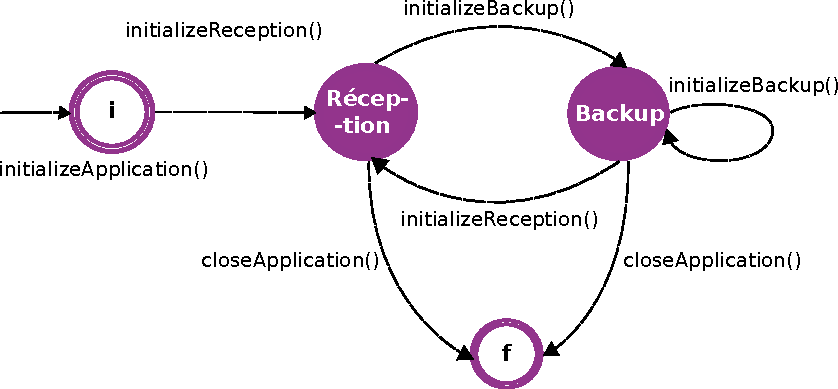
\includegraphics[width=.7\linewidth]{figures/state_machine}  
  \captionof{figure}{Machine à état de l'application Qt}
  \label{fig:stateMachine}
\end{figure}

D'un point de vue formel, le fonctionnement de l'application est régi par une machine à états relativement simple, représentée figure \ref{fig:stateMachine}.
Ces états facilitent la gestion des instances utiles à n'importe quel instant de l'exécution en dissociant clairement ce qui est du ressort de chacun des modes de fonctionnement définis. 
Le mode \emph{Réception} satisfait l'exigence principale du projet, à savoir présenter en temps-réel les résultats de \gls{SLAM} tout en assurant le contrôle du robot. 
Le mode \emph{Backup} répond à une fonctionnalité additionnelle offrant la possibilité à l'utilisateur de rejouer des données précédemment enregistrées. 
Le passage d'un état à l'autre est symbolisé par des flèches portant le nom de la méthode invoquée à cet effet.
Ces méthodes visent à libérer la mémoire relative au ressources dynamiques du mode courant, à instancier correctement les ressources graphiques ou de contrôle propres au mode requis et finalement, à changer une variable représentant 
l'état du système. 
On note que les fonctions de transition sont des slots atteint par des interactions spécifiques de l'utilisateur sur la fenêtre graphique. 

\begin{figure}[h]
  \makebox[\textwidth][c]{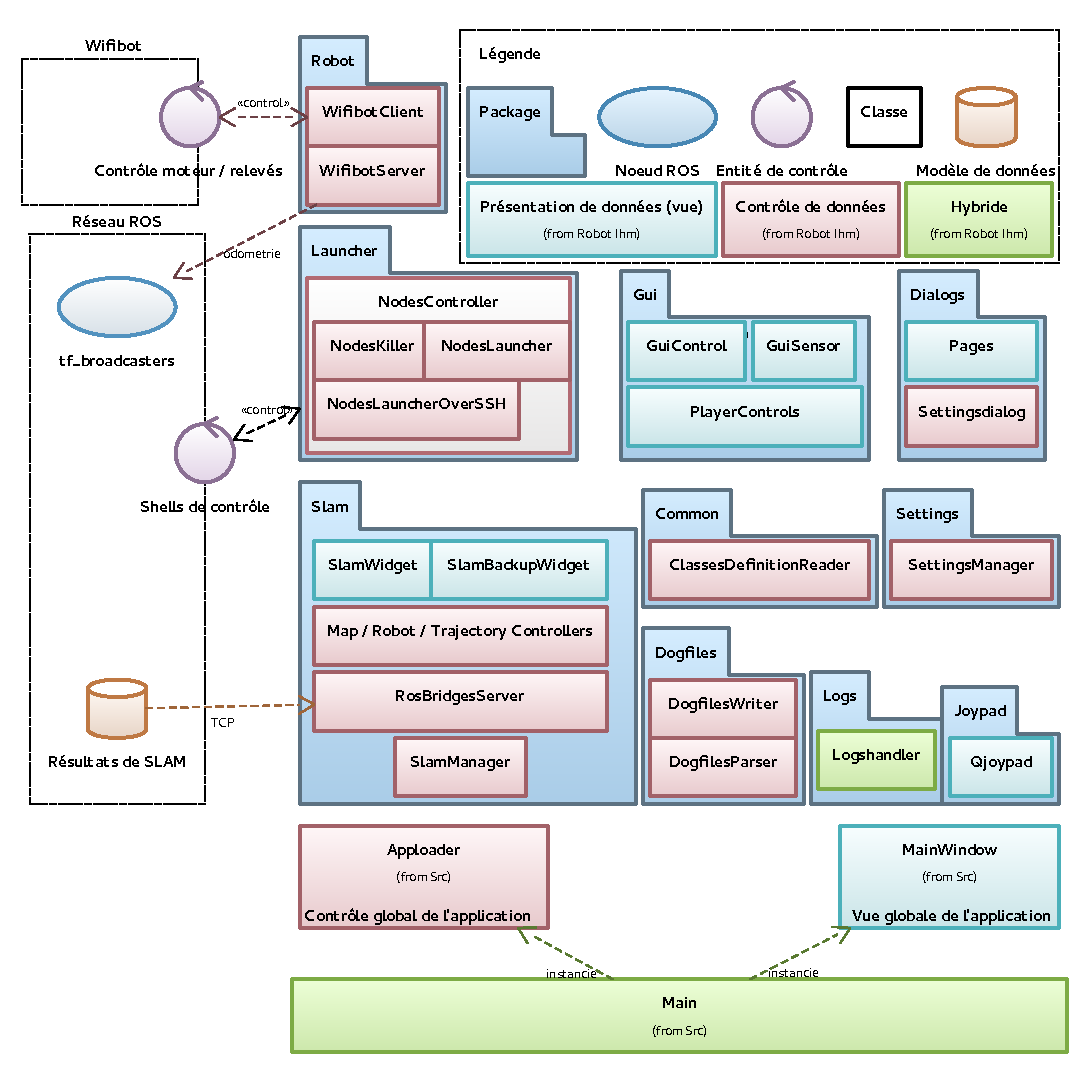
\includegraphics[width=1.1\textwidth]{figures/ihm-model}}%
  \captionof{figure}{Modèlisation logicielle de l'Interface Homme-Machine}
  \label{fig:modelIHM}
\end{figure}

La figure \ref{fig:modelIHM} expose quant à elle les classes et packages développés avec Qt pour répondre aux exigences fonctionnelles et d'interface précédemment formulées.   
Sont également représentés les moyens de communications mis en place entre l'IHM et les autres éléments constituant le projet : le réseau \gls{ROS} et la couche d'exploitation du Wifibot.

Le point d'entrée de l'application est la classe \path{main.cpp} qui instancie la fenêtre principale de l'application \path{MainWindow}\cite{Bib_qmainwindow} et une classe \path{Apploader} spécifique à notre architecture.
Cette dernière maintient et met à jour la machine à états présentée en \ref{fig:stateMachine} gérant ainsi le cycle de vie de toutes les autres instances.  

Le package \emph{SLAM} traite les données en sortie du réseau \gls{ROS}. 
La classe \path{ROSBridgesServer} instancie un serveur \gls{TCP} consacré à la communication avec les n\oe{}uds de bridges décrits dans la partie \ref{subsection:ROSnodes}. 
Ces données sont ensuite transmises à des contrôleurs dédiés à chaque type de données (carte, position ou trajectoire) qui assurent le parsing des paquets reçus puis émettent des signaux aux \emph{widgets} de rendu. 
Dans notre cas, deux \emph{widgets} sont susceptibles de rendre ces données : \path{SlamWidget} ou \path{SlamBackupWidget} respectivement associés au mode \emph{Réception} ou \emph{Backup}.
Ces \emph{widgets} héritent de la classe Qt \emph{QOpenGLWidget} fournissant les fonctionnalités de rendu graphique d'OpenGL dans un contexte Qt. 
La figure \ref{fig:reception} donne un apperçu de l'\gls{IHM} en mode \emph{Réception} afin de présenter les différents éléments de l'application. 
La fidélité des résultats sera quant à elle discutée dans la partie \ref{chap:bilan}.  

\begin{figure}[h]
  \centering
    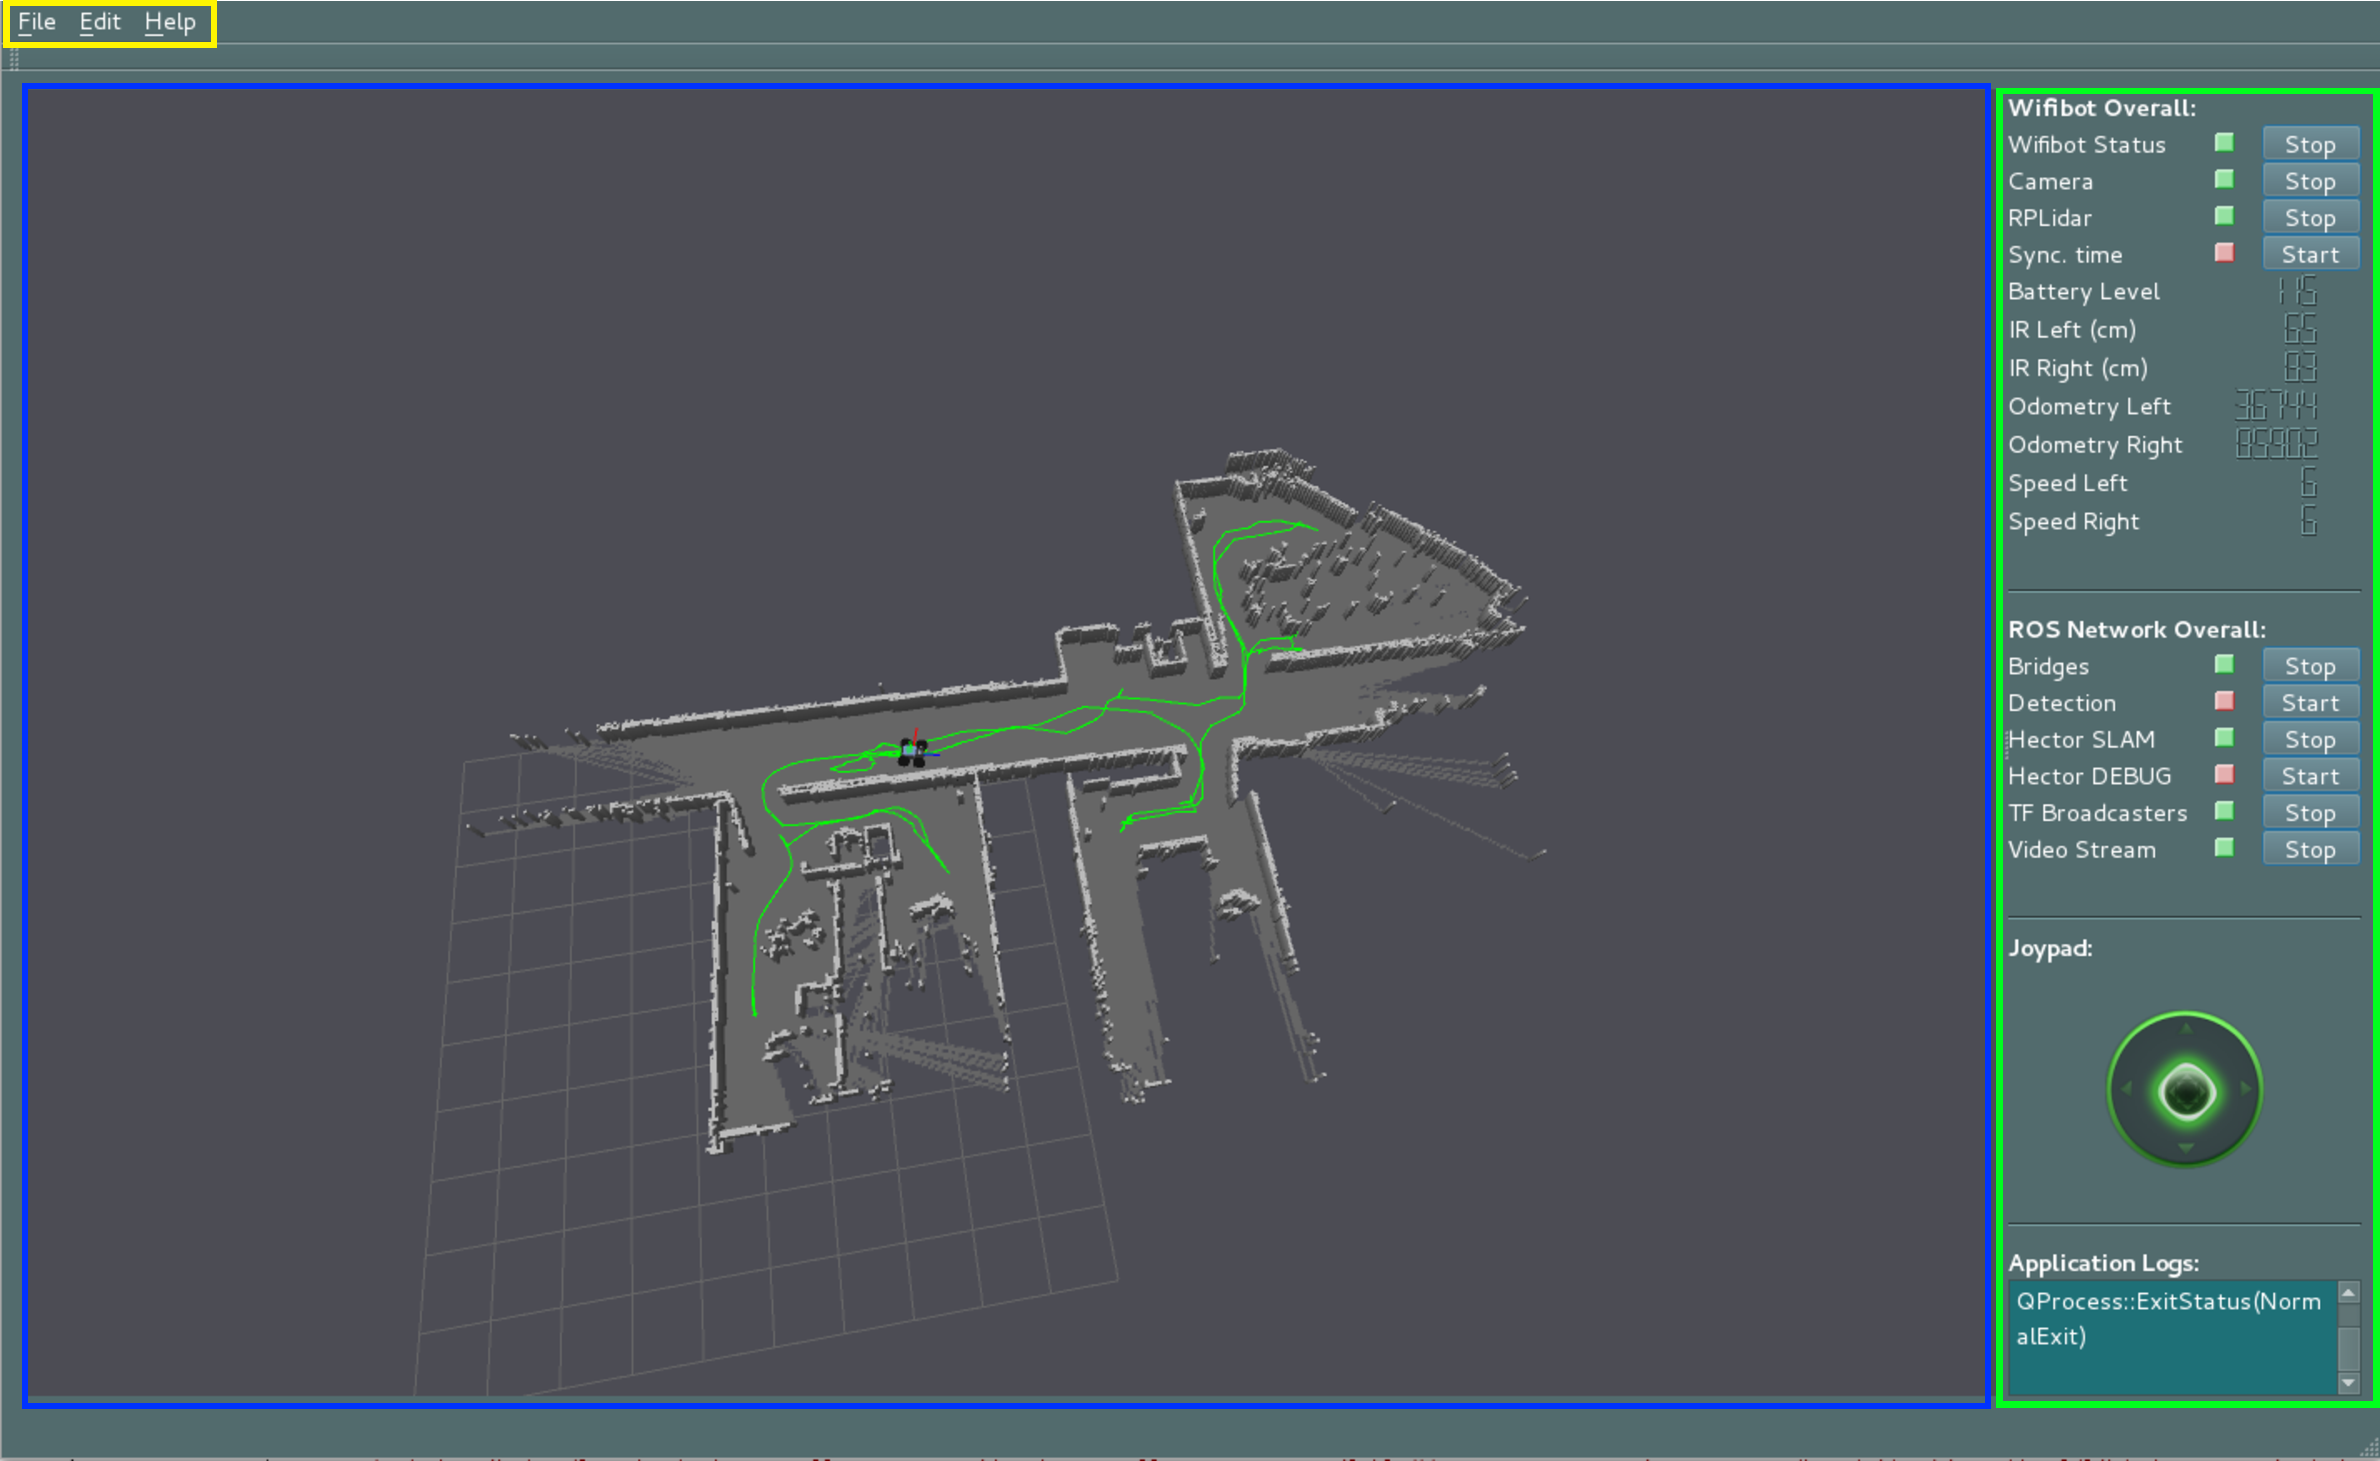
\includegraphics[width=1.\linewidth]{figures/slam-widget}  
  \captionof{figure}{Rendu visuel de l'IHM en mode Réception}
  \label{fig:reception}
\end{figure}

Nous pouvons visualiser la fenêtre principale (\path{MainWindow}) complétée d'instances de \emph{widgets} responsables du rendu d'éléments d'intérêt : 
\begin{itemize}
 \item \textbf{un widget de rendu OpenGL}, en bleu, fourni une représentation de la carte, du robot par le biais d'un modèle 3D et de sa trajectoire (position et orientation en tout temps)
 \item \textbf{un panneau de contrôle}, en vert, est découpé en quatre sections : le Wifibot, le réseau ROS, un joystic virtuel et une console de logs 
 \item \textbf{une barre de menu}, en jaune, permet la sauvegarde de jeux d'acquisition, le chargement d'une sauvegarde pour la rejouer, l'édition de paramètres de l'application ou l'affichage du manuel utilisateur
\end{itemize}

La figure \ref{fig:replay} expose le rendu global en mode \emph{Backup}. 
Celui-ci se distingue particulièrement du mode d'acquisition par la présence --au sein du panneau de contrôle-- d'un \emph{player} offrant les fonctionnalités d'un lecteur multimédia classique.

\begin{figure}[h]  
  \centering
    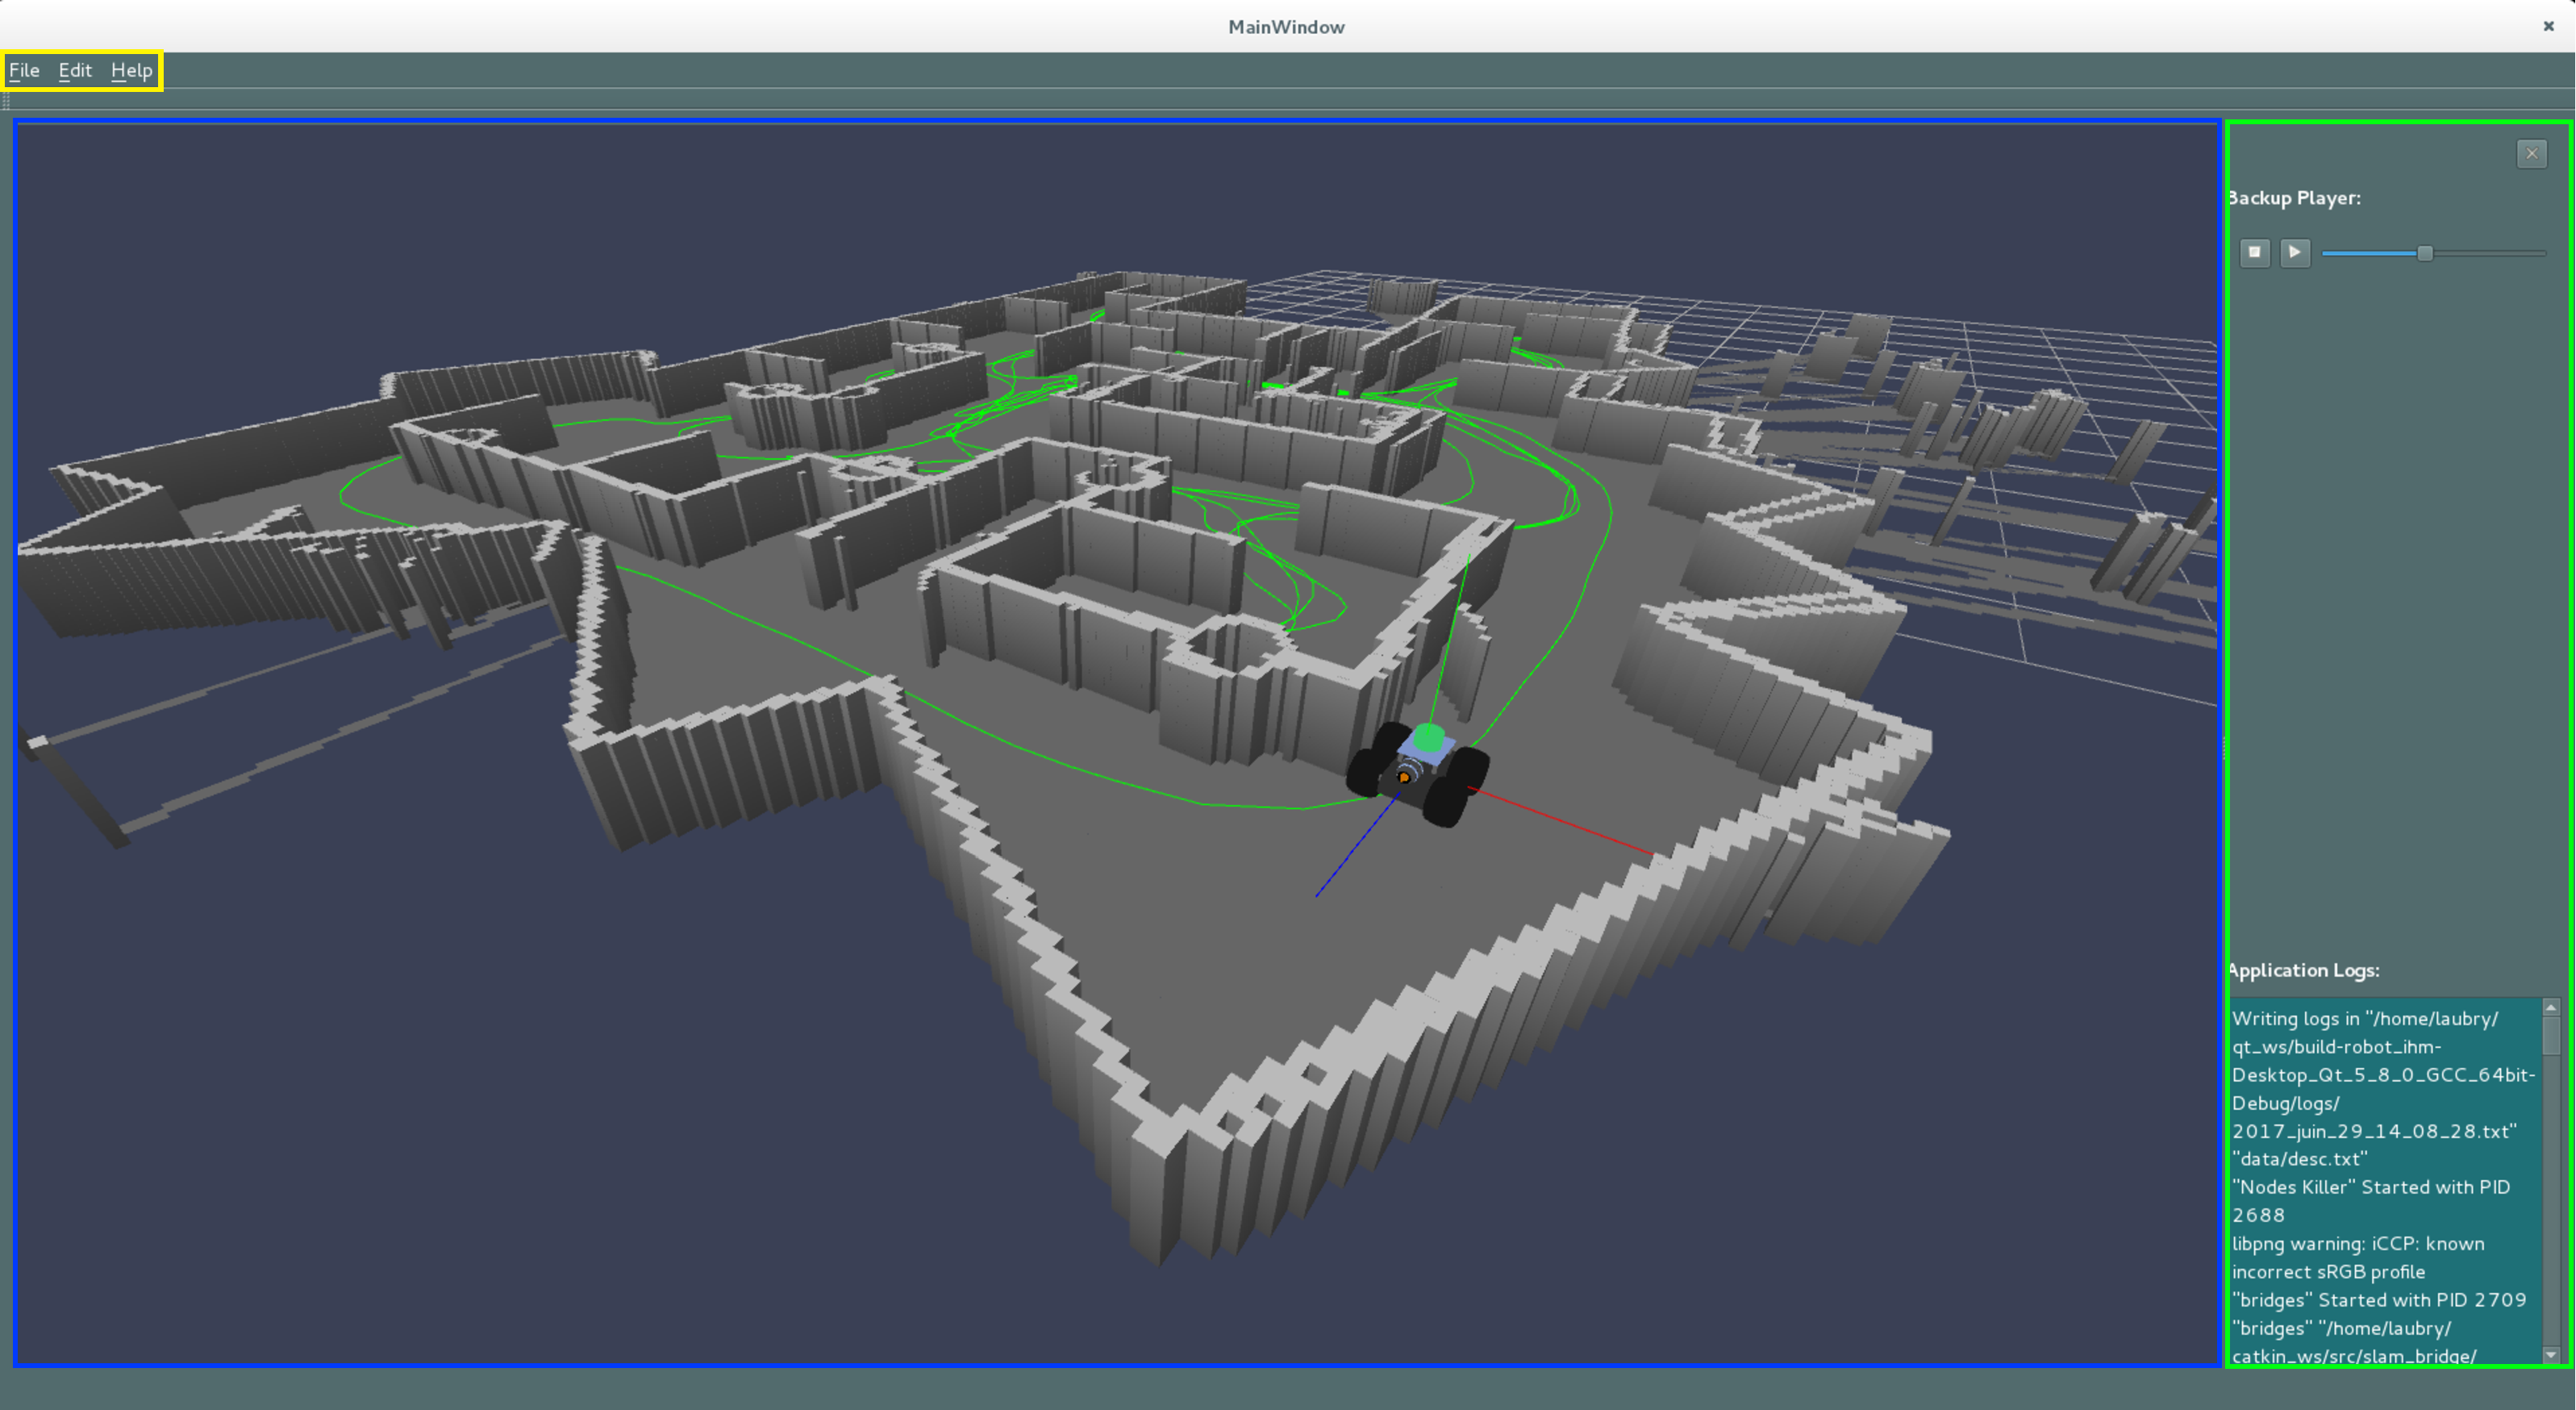
\includegraphics[width=1.\linewidth]{figures/slam-backup}  
  \captionof{figure}{Rendu visuel de l'IHM en mode rejeu}
  \label{fig:replay}
\end{figure}

\`{A} cet effet, un format d'enregistrement des données propre à l'application à été défini en \gls{XML}.
Ce format, appelé \emph{DOG}\footnote{Pour Detection and Occupancy Grid} est géré par les classes du package \path{DogFiles} : \path{DogFilesWriter} pour l'écriture et \path{DogFilesParser} pour la lecture. 
Des techniques de compressions ont été mises en \oe{}uvre pour les données de taille critique devant être sauvegardées. 
Ainsi, les données décrivant la carte sont traitées par un algorithme d'encodage par répétition (Run Lenght Encoding) tandis que toutes les composantes des vecteurs de trajectoire du robot sont gérées par la méthode suivante :

\begin{lstlisting}[style=customcpp]
// Multiply entry by 100, truncate it and returns its hexadecimal value. Negative number are concatenated with '-' char and encoded like positive values.
QString SlamWidget::floatToHex(float v)
{
    return (int)(v * 100) >= 0.0f
            ? QString::number( (int)(v * 100), 16 )
            : QString('-' + QString::number( (int)-(v * 100), 16 ));
}
\end{lstlisting}

Un algorithme similaire a été appliqué pour l'ensemble des orientations du robot. 
Ces techniques ont permis de réduire significativement les données à sauvegardées à l'aide d'une compression sans perte dans un  premier cas et une perte de l'ordre du centième de case (soit 0.0005m) dans un second cas.  
  
  \subsection{\'{E}léments de modularité mis en place}
  
La réalisation de l'application a d'emblée été associée à un objectif de modularité afin d'appréhender au mieux la perspective de stages futurs et / ou d'une possible adaptation industrielle du projet. 
L'utilisation de ROS allant dans ce sens, il paraissait intéressant d'appliquer cet état d'esprit à l'\gls{IHM}, tant dans l'architecture du logiciel que dans les fonctionnalités proposées à l'utilisateur final. 

Le premier point se retrouve principalement dans l'implémentation de l'\path{Apploader} qui gère le cycle de vie des instances d'une manière communément compréhensible : création, mise-à-jour puis destruction.  
D'autre part, l'interface graphique et les éléments de communication avec les n\oe{}uds peuvent eux-même être modifiés à convenance par le biais de l'\gls{IHM}. 
Nous exposons ici les principes qui sous-tendent cette démarche, nous amenant à balayer les points suivants : 

\begin{itemize}
  \item le paramétrage modulaire du réseau ROS
  \item les éléments graphiques attestant l'état de chaque n\oe{}ud
  \item le contrôle du réseau ROS depuis l'IHM
\end{itemize}

Qt offre un système de paramétrage des applications s'appuyant sur des fichiers au format texte et d'une classe \path{QSettings} indépendante de la plateforme utilisée
\footnote{En l'occurence, sur un système Unix, de tels fichiers seront stockés au format \path{.ini} sous \path{~/.config/<filename>.ini}}.
Cette dernière permet l'écriture de paramètres selon le paradigme clé / valeur et hiérarchisés sous forme de groupe.  
Dans notre IHM, une classe statique \path{SettingsManager} est utilisée pour écrire de tels paramètres, soit à l'initialisation de l'application soit lors de la configuration de celle-ci par l'utilisateur. 
Nous avons défini les groupes suivants relativement au réseau ROS :

\renewcommand*\DTstylecomment{\rmfamily\color{red}}
\dirtree{%
.1 ros\DTcomment{groupe de paramétrage du réseau ROS}. 
.2 $<$ID$>$\DTcomment{identifiant du groupe de paramètres}. 
.3 package. 
.4 $<$nom du package$>$\DTcomment{nom du package à invoquer}. 
.3 lauchfile. 
.4 $<$launchfile$>.$launch\DTcomment{nom du launchfile à invoquer}. 
.3 islocalnode. 
.4 $<$bool$>$\DTcomment{indique si le noeud est local ou embarqué}. 
.3 label. 
.4 $<$GUI label$>$\DTcomment{label à afficher sur l'interface}. 
.3 nodes. 
.4 node. 
.5 $<$liste de noeuds$>$\DTcomment{liste de noeuds à stopper}. }

L'utilisateur peut mettre à jour ou supprimer les valeurs par défaut et créer de nouvelles entrées directement depuis l'application sous \path{Edit > Settings > ROS} (voir figure \ref{fig:settings}).

\begin{figure}[h]
  \centering
    
\includegraphics[width=.7\linewidth]{figures/settings}  
  \captionof{figure}{Boîte de dialogue de configuration du réseau ROS depuis l'IHM}
  \label{fig:settings}
\end{figure}

Ces paramètres sont ensuite parsés, permettant la présentation et l'utilisation de chaque module ROS de manière uniforme.
D'un point de vue graphique, la classe \path{GuiControl} est responsable de la création dynamique des éléments de l'interface représentant les modules ROS, à partir de la clé de configuration \path{ros/<ID>/label/<GUI label>} 
tels que représentés figure \ref{fig:guicontrols}.

\begin{figure}
  \centering
    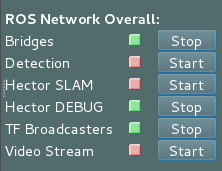
\includegraphics[width=.3\linewidth]{figures/guicontrols}  
  \captionof{figure}{Contrôle du réseau ROS créé dynamiquement sur l'interface graphique}
  \label{fig:guicontrols}
\end{figure}

Parallèlement, chaque nouvel identifiant sous \path{ros/<ID>} entraine l'instanciation de la classe \path{NodesLauncher} ou \path{NodesLauncherOverSSH} --en fonction du caractère local ou non du package-- et de la classe 
\path{NodesKiller}. 
Ces objets exécutent un shell Linux (\path{/bin/bash}) au sein d'un membre Qt de type \path{QProcess} permettant l'éxecution du launchfile afférent lorsque l'utilisateur presse le bouton ``Start'' du module.
Ils sont aussi responsables de la redirection des sorties du processus vers les sorties dédiées à la journalisation des évènements de l'application\footnote{La classe \path{LogsHandler} est utilisée pour journaliser les messages d'une part dans des fichiers datés du répertoire d'exécution 
de l'application et d'autre part, dans la console du panneau de contrôle}. 
La classe \path{NodesKiller} va quant à elle émettre des commandes système vers le ROS Master afin de tuer les n\oe{}uds d'un package lorsque l'utilisateur souhaitera mettre fin à leur exécution. 

Pour résumer, un utilisateur voulant ajouter un nouveau package ROS à l'application devra le compiler de manière classique dans son workspace catkin, éditer un launchfile permettant d'éxecuter le ou les n\oe{}uds afférents puis
simplement renseigner les informations requises depuis l'IHM. 
Sous la section \path{Edit > Settings > Network} l'utilisateur pourra également configurer les noms d'hôtes et adresses IP distants, adaptant ainsi le système à d'autres modèles ou instances de robots. 
Si l'opérateur venait à utiliser une plateforme dotée de capteurs communiquant leurs résultats à un package ROS dédié, le contrôle de ces nouveaux éxecutables pourrait être couvert par l'application en quelques manipulations seulement.  